\chapter{Implementation}
\label{chap:implementation}

Something about libuv and how it is very convenient to prototype async stuff


\begin{figure}[h]
    \centering
    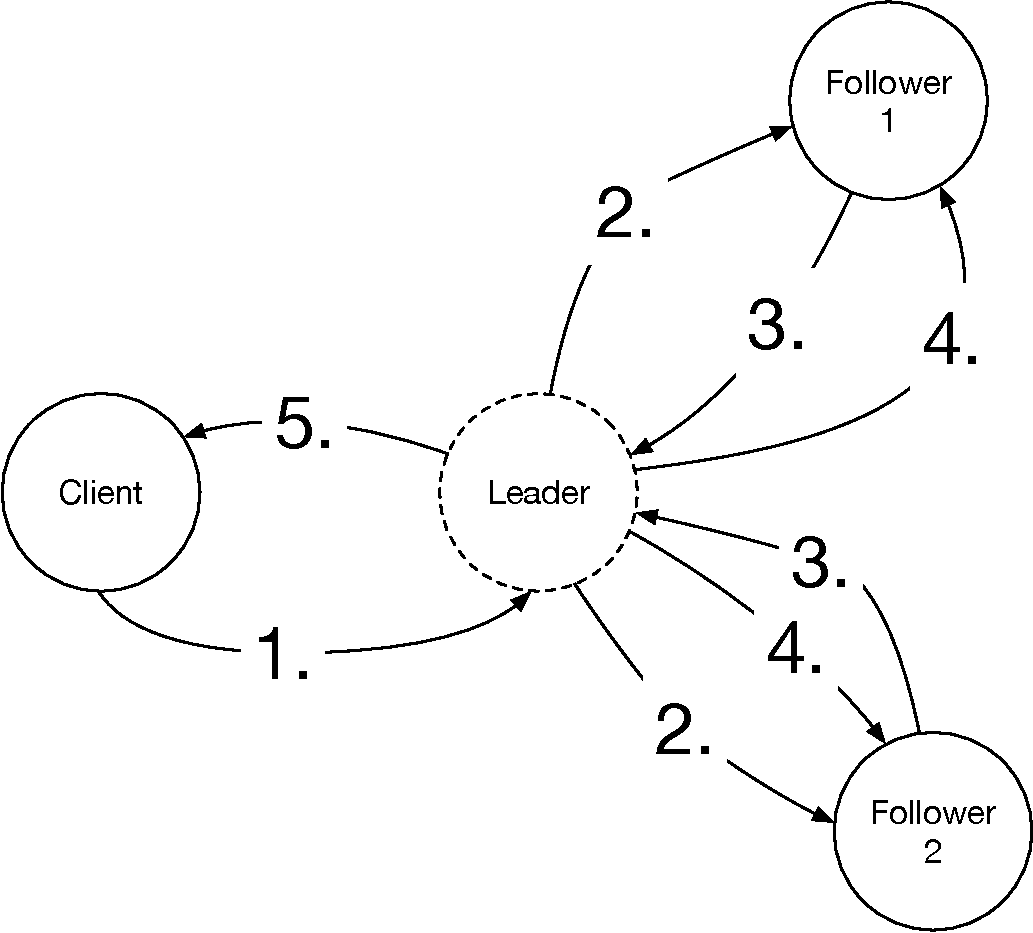
\includegraphics[width=0.8\textwidth]{client_server_interaction}
    \caption{Typical client server interaction for a replicated service call.
        1. The request is sent from the client to the leader.
        2. The leader replicates the request to all followers.
        3. The followers acknowledge the replication.
        4. Once the request is replicated on a majority of servers the leader commits it.
        5. The commited request is sent to the application (on every node) and then the reply is sent back to the client.
    \label{fig:client-server-interaction}
    }
\end{figure}

\section{Choice of a consensus protocol}

One of the earliest solution to the consensus problem is Lamport's Paxos algorithm\cite{paxos}.
It is currently widely used, for example Google relies on it a lot to ensure correctness of its distributed systems\cite{chubby, paxoslive}.
However, Paxos has two issues: first, it only solves part of the problem; some other ``bricks'' must be added to it to form a complete system.
In addition to this, Paxos is known to be hard to understand, and even more to implement correctly.
Most of its user rely on pre-existing implementations such as libpaxos\footnote{\url{https://bitbucket.org/sciascid/libpaxos/}}.
This means modifying the consensus protocol for our application and chosent transport could be hard to do

Fortunately for us, a simpler alternative to Paxos called Raft was recently introduce\cite{raft}.
Raft was designed from the ground up to be simpler by cleanly separating the different parts of the problem.
It also provides a complete solution, unlike Paxos which often requires additional, unproven extension\cite{paxoslive}.

Another possible choice would have been ZooKeeper's ZAB\cite{zookeeper}, but was not as well documented as Raft.
In addition, it appeared to provide primitives that were less general purposes than a replicated log.

Despite the availability of excellent production grade Raft implementations, we decided to implement our own.
Most existing Raft implementations are using high level languages such as Go, which are not suited for low latency programming.
Other implementations in C or C++ make a lot of hypothesis on the underlying platform.
For all those reasons, it was deemed easier to do it ourself, using experience gathered by doing a prototype in Python.
The resulting implementation is pretty small, at about 1000 lines of C++ code.

\section{Implementation language}

We initially planned to write the Raft prototype in Rust, using the NetBricks\cite{netbricks} framework.
The goal was to use Rust high level constructs to have compile time safety guarantees while maintaining good performance.
However, it turned out that using Rust for this project was less than ideal for several reasons.

NetBricks\cite{netbricks} is a Rust framework that provides everything needed to write high performance network applications in Rust.  % TODO: Something about Ogier writing R2P2 to rust
It provides a full userland networking stack, from the DPDK bindings up to UDP socket implementation.
Thanks to Rust's move semantics, NetBricks is capable of achieving zero copy processing of incoming packets, leading to very high performance.
Unfortunately, it does not appear to be developped actively anymore, which is an issue due to the fast evolving nature of the language.
The R2P2 Rust implementation\cite{ogier} written by another Master student appears to be incomplete at the moment.

Another issue with Rust was that the current ``reference'' implementation of R2P2 is written in C using a custom userland UDP/IP stack.
This means that the Rust / NetBricks code would have been difficult to integrate in the existing codebase, maybe even requiring a C rewrite.

Due to all those factors, we decided to switch the implementation strategy to directly writing code that could be used in C.
We use C++14, which is a lot more expressive than pure C.
Move semantics are also available in this language since C++11.
While not as useful as Rust's, mostly due to the lack of safety guarantees, they still form a very useful tool to reduce packet copying.

\section{Message serialization}

% TODO: is it really interesting ?

\begin{itemize}
    \item Custom code vs Protobuf
\end{itemize}



\section{Message Routing}

In Raft, only the leader can send new mesasges.
This keeps the protocol simpler by only having data flowing from the leader to the followers.
On the other hand, it means that we must also have a way to direct client queries to the leader.

In the original Raft paper\cite{raft}, the followers will redirect clients to the leader if contacted directly.
However, this is not optimal from a tail latency perspective: a client that picks a follower as a destination will see an additional \gls{rtt} to its request.

Fortunately, \gls{r2p2} was implemented with load balancing semantics in mind.
We can therefore extend the \gls{r2p2} load balancer to always propagate replicated requests to the current leader.
While this haven't been done yet, it could be implementing by having the load balancer listening to Raft heartbeat messages.

For our benchmarking we manually pointed the benchmark client to the elected leader.

\section{Log}

RAM based

Each element is one request

\section{DPDK}

\section{Userland implementation}

While kernel bypass offers the best performance, it is not always possible to use it (i.e. when using a \gls{nic} is shared between applications).
Our current implementation can therefore either be compiled to use DPDK (and a custom UDP/IP stack) or to use the kernel networking facilities.
In this second case, only \gls{r2p2} is implemented in the application; the rest runs in-kernel.

To achieve high performance and stay close to DPDK's event based model, we use asynchronous I/O facilities.
Our first implementation used Linux's \texttt{epoll} directly, making it non-portable.
We rewrote it to use libuv instead, which abstracts the different asynchronous I/O mechanisms on Linux, BSD and Windows.

This means that the current implementation can run as a normal networked component on all major platforms.
This allows for a much easier development experience than running DPDK directly, and can even be used in production with good performance.
